\documentclass[a4paper, 12pt]{article}


\usepackage[french]{babel}
\usepackage[utf8]{inputenc}
\usepackage[T1]{fontenc}
\usepackage{lmodern}
\usepackage{listings}
\usepackage{graphicx}
\usepackage{amsmath}
\usepackage{amsfonts}
\usepackage{amssymb}
\usepackage{caption}
\usepackage{subcaption}
\usepackage[usenames,dvipsnames]{xcolor}


\setcounter{secnumdepth}{4}
% TAILLE DES PAGES (A4 serré)

\setlength{\parindent}{0pt}
\setlength{\parskip}{1ex}
\setlength{\textwidth}{17cm}
\setlength{\textheight}{24cm}
\setlength{\oddsidemargin}{-.7cm}
\setlength{\evensidemargin}{-.7cm}
\setlength{\topmargin}{-.5in}

% Commandes de mise en page
\newcommand{\fichier}[1]{\emph{#1}}
\newcommand{\nom}[1]{\emph{#1}}
\newcommand{\Fig}[1]{Fig \ref{#1} p. \pageref{#1}}
\newcommand{\itemi}{\item[$\bullet$]}

% Commandes de maths
\newcommand{\fonction}[3]{#1 : #2 \to #3}
\newcommand{\intr}[2]{\left[ #1 ; #2 \right]}
\newcommand{\intn}[2]{\left[\![ #1 ; #2 \right]\!]}
\newcommand{\intro}[2]{\left] #1 ; #2 \right[}
\newcommand{\intrsod}[2]{\left[ #1 ; #2 \right[}
\newcommand{\ps}[2]{\langle #1, #2 \rangle}
\newcommand{\mdelta}[1]{\boldsymbol{\delta_{#1}}}
%% \newcommand{\mdelta}[1]{\delta_{\textbf{#1}}}

\pagenumbering{arabic}
\graphicspath{{images/}}

\title{ASM-TP1 : Cancer de la prostate} 
\author{Pierre Petitbon \and Florian Privé \and Xinrui Xu}
\date{}

\begin{document}

\maketitle

\section{Analyse préliminaires des données}

\begin{enumerate}

\item On visualise sous R la matrice de corrélation entre lpsa et les 8 prédicteurs. 

\begin{center}
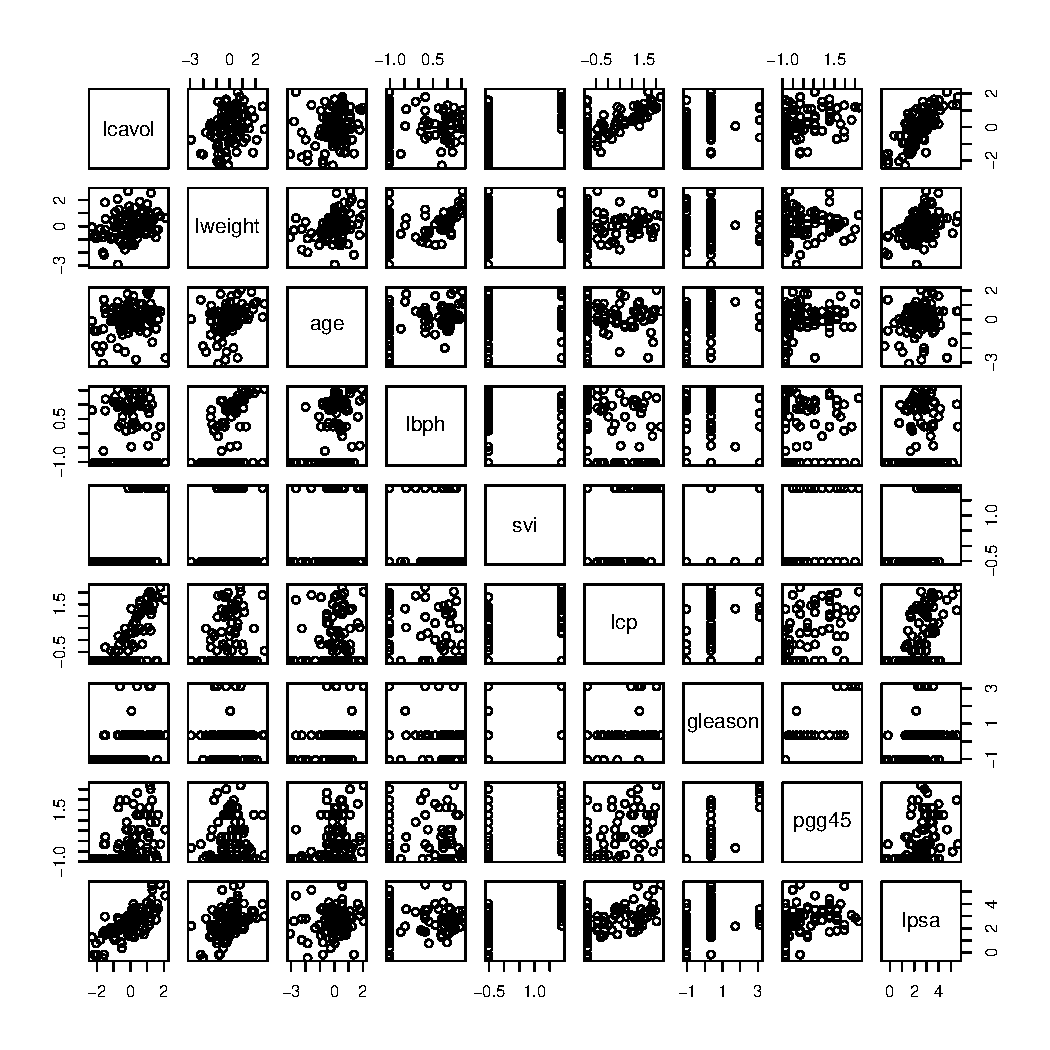
\includegraphics[scale=0.5]{Rplots.pdf}
\captionof{figure}{Rplots}
\label{fig1}
\end{center}

À partir du graphe précédent, on peut voir que certains facteurs sont corrélés ou pas avec lpsa. Pour cela, il suffit de regarder si le nuages de points forme plus ou moins une ellipse. 

\begin{tabular}{|p{0.5cm}|p{1.5cm}|p{1.5cm}|p{1.5cm}|p{1.5cm}|p{1.5cm}|p{1.5cm}|p{1.5cm}|p{1.5cm}|}
  \hline
       & lcavol & lweight & age & lbph & svi & lcp & gleason & pgg45 \\
  \hline
  lpsa & corrélé & non 

   corrélé & non 

    corrélé & non

     corrélé & corrélé & corrélé & non

      corrélé & non

       corrélé \\
  \hline 
\end{tabular}


\item 
À partir du graphe précédent, on peut aussi conjecturer s'il y a corrélation entre les prédicteurs.

\begin{tabular}{|p{1.4cm}|p{1.4cm}|p{1.4cm}|p{1.4cm}|p{1.4cm}|p{1.4cm}|p{1.4cm}|p{1.4cm}|p{1.4cm}|p{1.4cm}|}
  \hline
       & lcavol & lweight & age & lbph & svi & lcp & gleason & pgg45 \\
  \hline
  lcavol &  & non 

  corrélé & non 

   corrélé & corrélé & corrélé & corrélé & corrélé & corrélé \\
  \hline 
  lweight & non 

  corrélé & & non

  corrélé & non

  corrélé & non 

  corrélé & corrélé & corrélé & non

   corrélé \\
   \hline
   age & non 

   corrélé & non 

   corrélé &  & corrélé & corrélé & non 

   corrélé & corrélé & non 

   corrélé \\
   \hline
   lbph & corrélé & non 

   corrélé & corrélé & & corrélé & 
   non 

   corrélé & non 

   corrélé &
   non

   corrélé \\
   \hline
   svi & corrélé & non 

   corrélé & corrélé & corrélé & & corrélé & non 

   corrélé & corrélé \\
   \hline
   lcp & corrélé & corrélé & non 

   corrélé & non 

   corrélé & corrélé &  & corrélé & non

    corrélé \\
    \hline
    gleason & corrélé & corrélé & corrélé & non 

    corrélé & non 

    corrélé & corrélé & & corrélé \\
    \hline
    pgg45 & corrélé & non 

    corrélé & non 

    corrélé & non 

    corrélé & corrélé & non 

    corrélé & corrélé & \\
    \hline

\end{tabular}

\end{enumerate}



\section{Régression linéaire. Méthodes des moindres carrés.}

\begin{enumerate}
\item
La régression classique consiste à estimer les coefficients $\beta_{j}$ intervenant dans la relation suivante :

$ Y_{i} = \sum\limits_{j=1}^6 \beta_{j} x_{ij} + \beta_{0} + \sum\limits_{l=2}^4 \beta_{gleason, l} \mathbf{1}_{x_{gleason, i}=l} + \epsilon_{i} $

où $Y$ représente lpsa et les $x_{j}$ représentent les prédicteurs.  

D'après les résultats obtenus, les prédicteurs qui semblent influer le plus sur lpsa sont :
\begin{itemize}
\item lcavol (***) : on prend un risque très faible (p-valeur $=2.9x10^{-8}\%$) en disant que $\beta_{lcavol} \neq 0$.
\item lweight (**) : p-valeur $=0.25\%$.
\item svi (**) : p-valeur $=0.31\%$.
\item age (*) : p-valeur $=4.4\%$.
\end{itemize}




\end{enumerate}

\section{Effet des prédicteurs quantitatifs}



\section{Sélection du meilleur sous-ensemble. Méthode «Best subscript selection»}

\begin{enumerate}

\item On ne peut se limiter à l'analyse du modèle en partie 2 car on garde tous les paramètres sans distinction. Il faudrait ne garder que les prédicteurs pertinents, qui ont une influence réelle sur lcavol. Certains prédicteurs ne servent qu'à approcher le bruit dans l'échantillon, ce qui permet effectivement de se rapprocher des données, mais cela dégrade la qualité des prédictions. On parle alors d'overfitting.

Autrement dit, le problème majeur est que le critère RSS est insuffisant : plus on a de prédicteurs, meilleure la régression est jugée. Or, les prédictions peuvent se détériorer lorsqu'on utilise des prédicteurs superflus qui ne servent qu'à approcher le bruit.

\item Pour chaque $k$ dans $\{0, ..., 8\}$, on fait varier le choix des prédicteurs afin de minimiser le RSS. La courbe des RSS ainsi obtenus vérifie bien la décroissance avec le nombre de prédicteurs. On observe un saut important à l'ajout du premier prédicteur (le RSS diminue de moitié), ce qui n'a rien d'étonnant : cela témoigne de l'intérêt de faire une régression. A l'ajout du deuxième puis du troisième prédicteur, le RSS diminue encore assez significativement, puis il reste presque inchangé au-delà.

\begin{figure}
\begin{center}
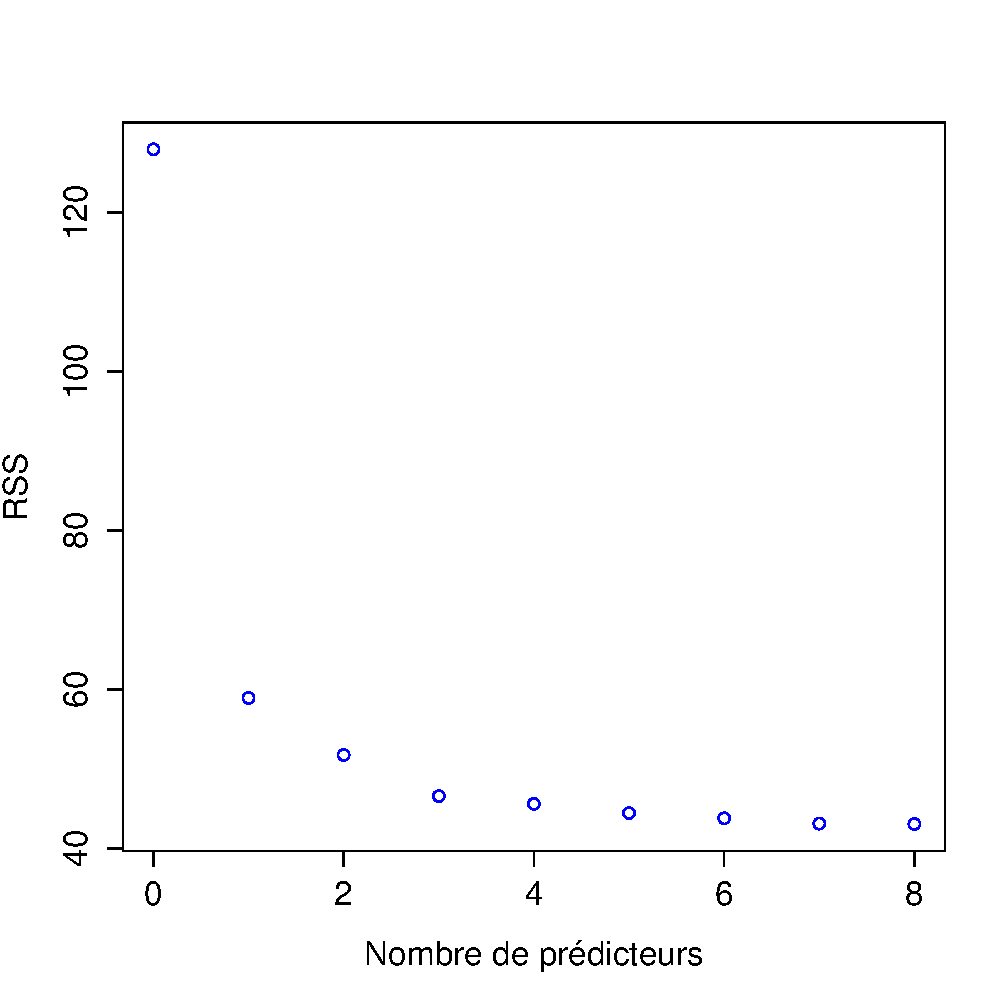
\includegraphics[scale=0.7]{rss.pdf}
\caption{Graphe des RSS en fonction du nombre de prédicteurs}
\end{center}
\end{figure}

On indique ci-dessous les sous-ensembles de prédicteurs qui réalisent le minimum de RSS, à nombre $k$ de prédicteurs fixé :
\begin{itemize}
\item $k = 0: \emptyset$
\item $k = 1: \{lcavol\}$
\item $k = 2: \{lcavol, lweight\}$
\item $k = 3: \{lcavol, lweigth, svi\}$
\item $k = 4: \{lcavol, lweight, lbph, svi\}$
\item $k = 5: \{lcavol, lweight, age, lbph, svi\}$
\item $k = 6: \{lcavol, lweight, age, lbph, svi, lcp\}$
\item $k = 7: \{lcavol, lweight, age, lbph, svi, lcp, pgg45\}$
\item $k = 8: \{lcavol, lweight, age, lbph, svi, lcp, gleason, pgg45\}$
\end{itemize}

\item Cette méthode ne permet pas de sélectionner le meilleur modèle, toutes tailles confondues, il ne permet que de déterminer le modèle qui "colle" le plus aux données, le nombre de prédicteurs étant fixé. Le meilleur modèle n'est pas nécessairement celui qui considère le plus de prédicteurs. En particulier, on n'évalue toujours pas la qualité des prédictions, qui est le seul critère qui importe véritablement. L'objectif de la split-validation est justement de tenir compte de ce critère pour affiner le choix du modèle.

\end{enumerate}


\section{Split-validation}

\begin{enumerate}

\item La split-validation consiste à séparer les échantillons en deux sous-ensembles :

\begin{itemize}
\item Une partie pour effectuer différentes régressions (ensemble d'apprentissage)
\item Une partie pour tester les différents modèles de régression possibles, et sélectionner celui qui produit les meilleures prédictions (ensemble de test)
L'ensemble de test permet donc de comparer les valeurs prédites aux valeurs mesurées.
\end{itemize}

\item 

\item Le meilleur modèle de taille 2 contient les prédicteurs $i = 1$ (lcavol) et $j = 2$ (lweight). lm(lpsa~.,data=pro[-valid,c(i,j,9)]) correspond au calcul de la régression sur l'ensemble d'apprentissage (-valid), en s'intéressant uniquement aux prédicteurs lcavol et lweight.

L'erreur d'apprentissage moyenne pour ce modèle est $0.503$. A noter que l'erreur est prise au sens des moindres carrés.

\item L'erreur de prédiction moyenne est $0.575$. On peut observer qu'elle est du même ordre de grandeur que l'erreur d'apprentissage moyenne.

\item En se basant sur cette unique split-validation, nous prendrions le modèle avec 2 prédicteurs. En effet, il s'agit du modèle qui minimise l'erreur de prédiction (cf. figure 3), qui est à nos yeux le critère essentiel pour juger d'un modèle de régression. Les deux prédicteurs retenus sont lcavol et lweight.

\item Le principal problème de la méthode de split-validation est la séparation arbitraire de l'échantillon en un ensemble d'apprentissage et un ensemble de test. Les résultats de la split-validation sont sensibles à cette séparation. En optant pour une séparation aléatoire des échantillons, la split-validation indique cette fois-ci qu'il faudrait prendre le modèle avec 3 prédicteurs car c'est à présent celui qui minimise l'erreur de prédiction (cf. figure 4).

\item Pour éviter ce problème, nous proposons d'itérer un nombre donné de fois (30 dans notre script) l'algorithme de split-validation avec séparation aléatoire de l'échantillon en deux moitiés de même taille. On récupère alors pour chaque itération les erreurs d'apprentissage et de prédiction moyennes. On calcule alors la moyenne de ces erreurs, et on se base sur ces résultats pour tirer des conclusions quant au choix du modèle. Les variations d'une itération à l'autre sont ainsi gommées. Avec cette méthode, on obtient que le meilleur modèle est celui avec 3 prédicteurs (cf figure 5).

\begin{figure}
\begin{center}
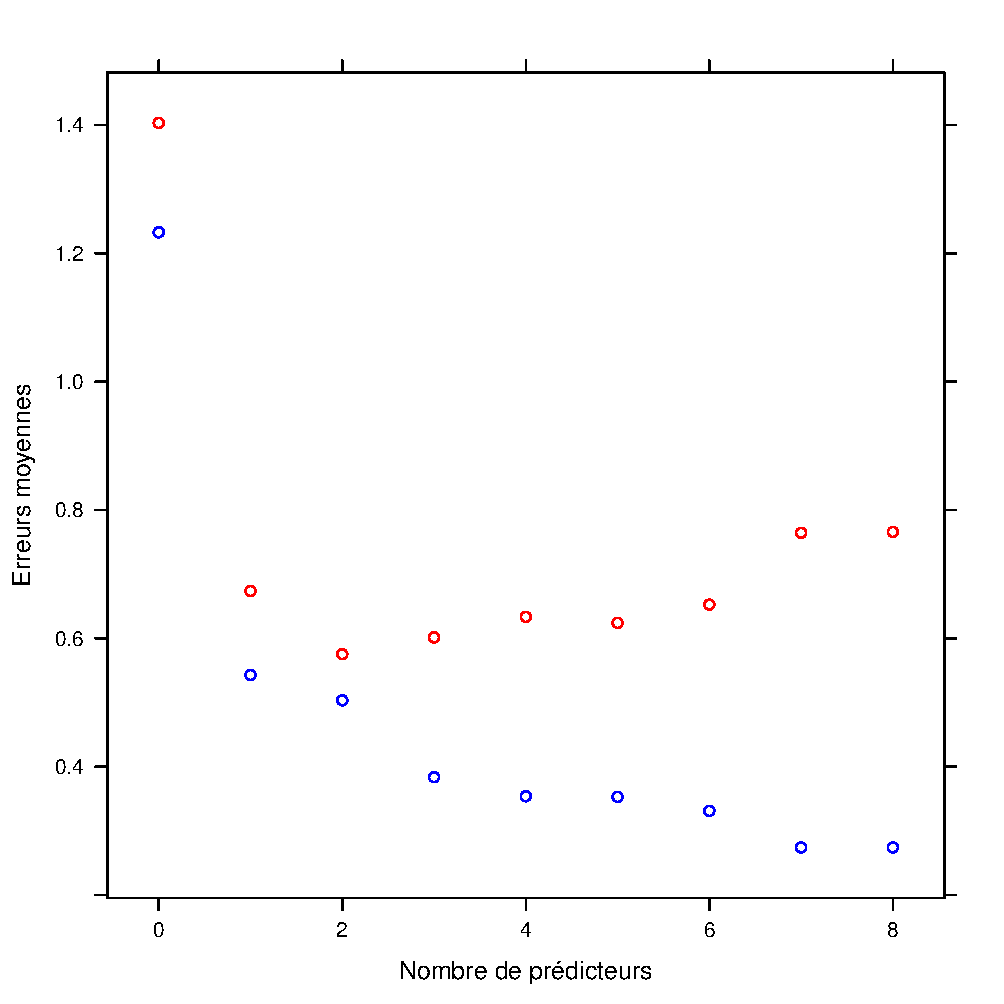
\includegraphics[scale=0.7]{erreurs_moy.pdf}
\caption{Tracé des erreurs d'apprentissage (en bleu) et de prédiction (en rouge) moyennes en fonction du nombre de prédicteurs}
\end{center}
\end{figure}

\begin{figure}
\begin{center}
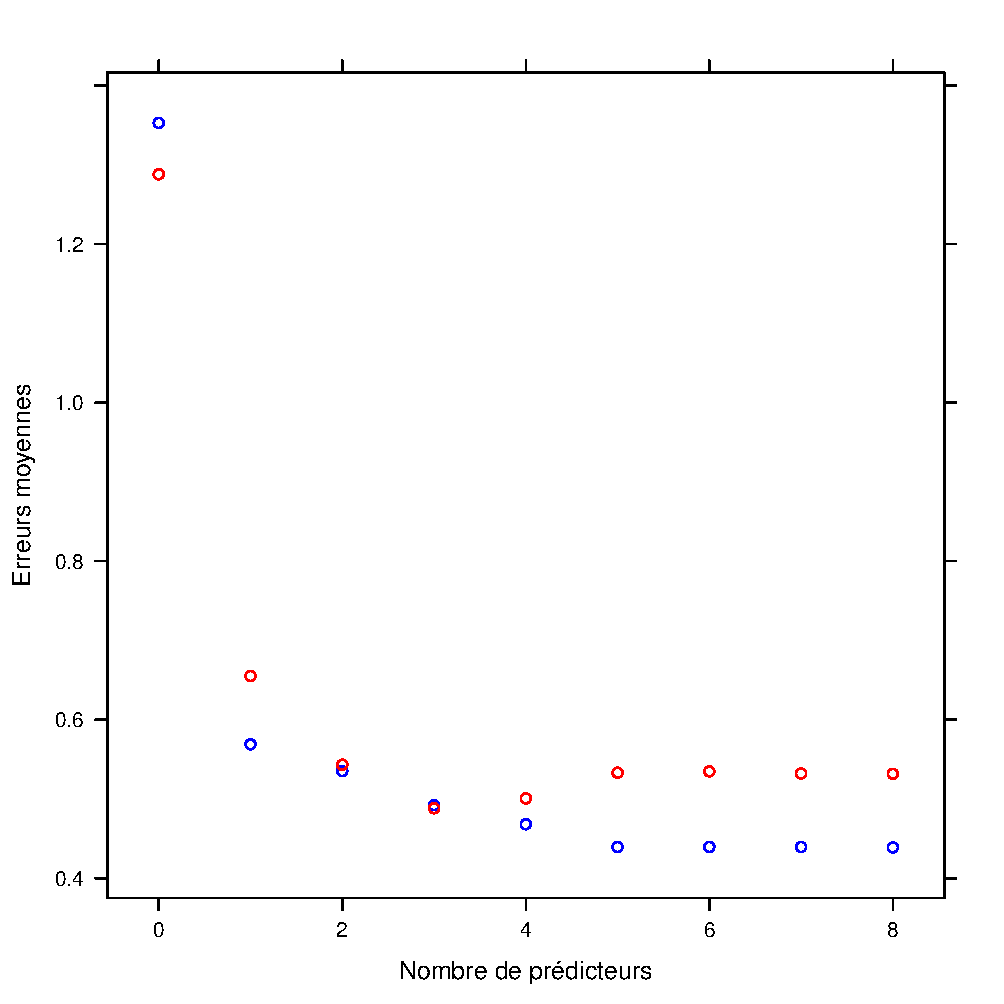
\includegraphics[scale=0.7]{erreurs_moy_autre.pdf}
\caption{Tracé des erreurs d'apprentissage (en bleu) et de prédiction (en rouge) moyennes pour une séparation aléatoire de l'échantillon}
\end{center}
\end{figure}

\begin{figure}
\begin{center}
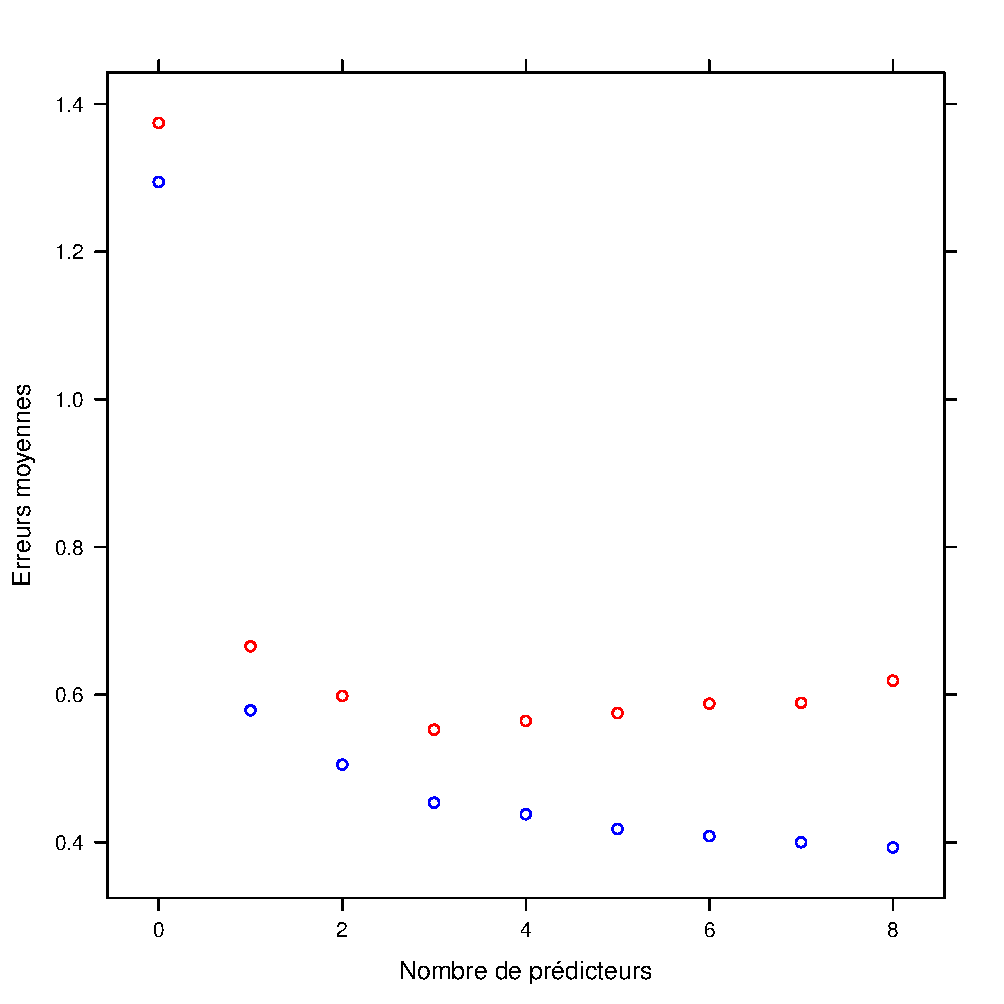
\includegraphics[scale=0.7]{erreurs_moy_moy.pdf}
\caption{Tracé des erreurs d'apprentissage (en bleu) et de prédiction (en rouge) moyennes sur 30 itérations avec séparation aléatoire}
\end{center}
\end{figure}

\end{enumerate}


\section{Conclusion}



\end{document}

% TODO : parler du scrum master
